\documentclass[conference]{IEEEtran}
\usepackage{microtype,mathtools,amsmath,multibib,amsfonts,multicol,array,multirow,place ins,cite,makecell,algorithm,algorithmic,subfigure,paralist,graphicx}
%\usepackage{flushend}

\usepackage[font=small,labelfont=bf]{caption}

\usepackage{xspace}
\usepackage{color}
\usepackage{ifthen}
\usepackage{url}
\usepackage{fancybox}


\graphicspath{{zu/}}
\DeclareGraphicsExtensions{.pdf,.jpeg,.png}
\hyphenation{op-tical net-works semi-conduc-tor}


\begin{document}
\title{Title}

\maketitle
\newboolean{showcomments}
\setboolean{showcomments}{true} % toggle to show or hide comments
\ifthenelse{\boolean{showcomments}}
{\newcommand{\nbnote}[2]{
  % \fbox{\bfseries\sffamily\scriptsize#1}
  \fcolorbox{blue}{yellow}{\bfseries\sffamily\scriptsize#1}
  {\sf\small\textit{#2}}
  % \marginpar{\fbox{\bfseries\sffamily#1}}
 }
}
{\newcommand{\nbnote}[2]{}
 \newcommand{\version}{}
}
\newcommand\pick[1]{\nbnote{Pick sez}{\textcolor{magenta}{#1}}}
\newcommand\thai[1]{\nbnote{Thai sez}{\textcolor{blue}{#1}}}


\begin{abstract}

% the freeform style of modern code review

% some comments are not technically contributing


\begin{IEEEkeywords}
Peer Code Review, Software Inspection, Reviewer Recommendation, Reviewer Assignment
\end{IEEEkeywords}
\end{abstract}

\section{Introduction}
Motivation Example.\thai{Wow}
\begin{description}
\item[RQ1:] Can we identify useful and useless discussions in code review?
\item[RQ2:] How impact of useless discussion impact to the software quality?
\end{description}

\section{Background}
\subsection{Modern Code Review}
\subsection{Text Mining Techniques}
\subsubsection{tf--idf}
\subsubsection{Similarity Measure}
\subsection{Evaluation Techniques}
\subsubsection{Precision and Recall}
\subsubsection{F-measure}


\section{Classification Method}

\begin{figure*}
\centering
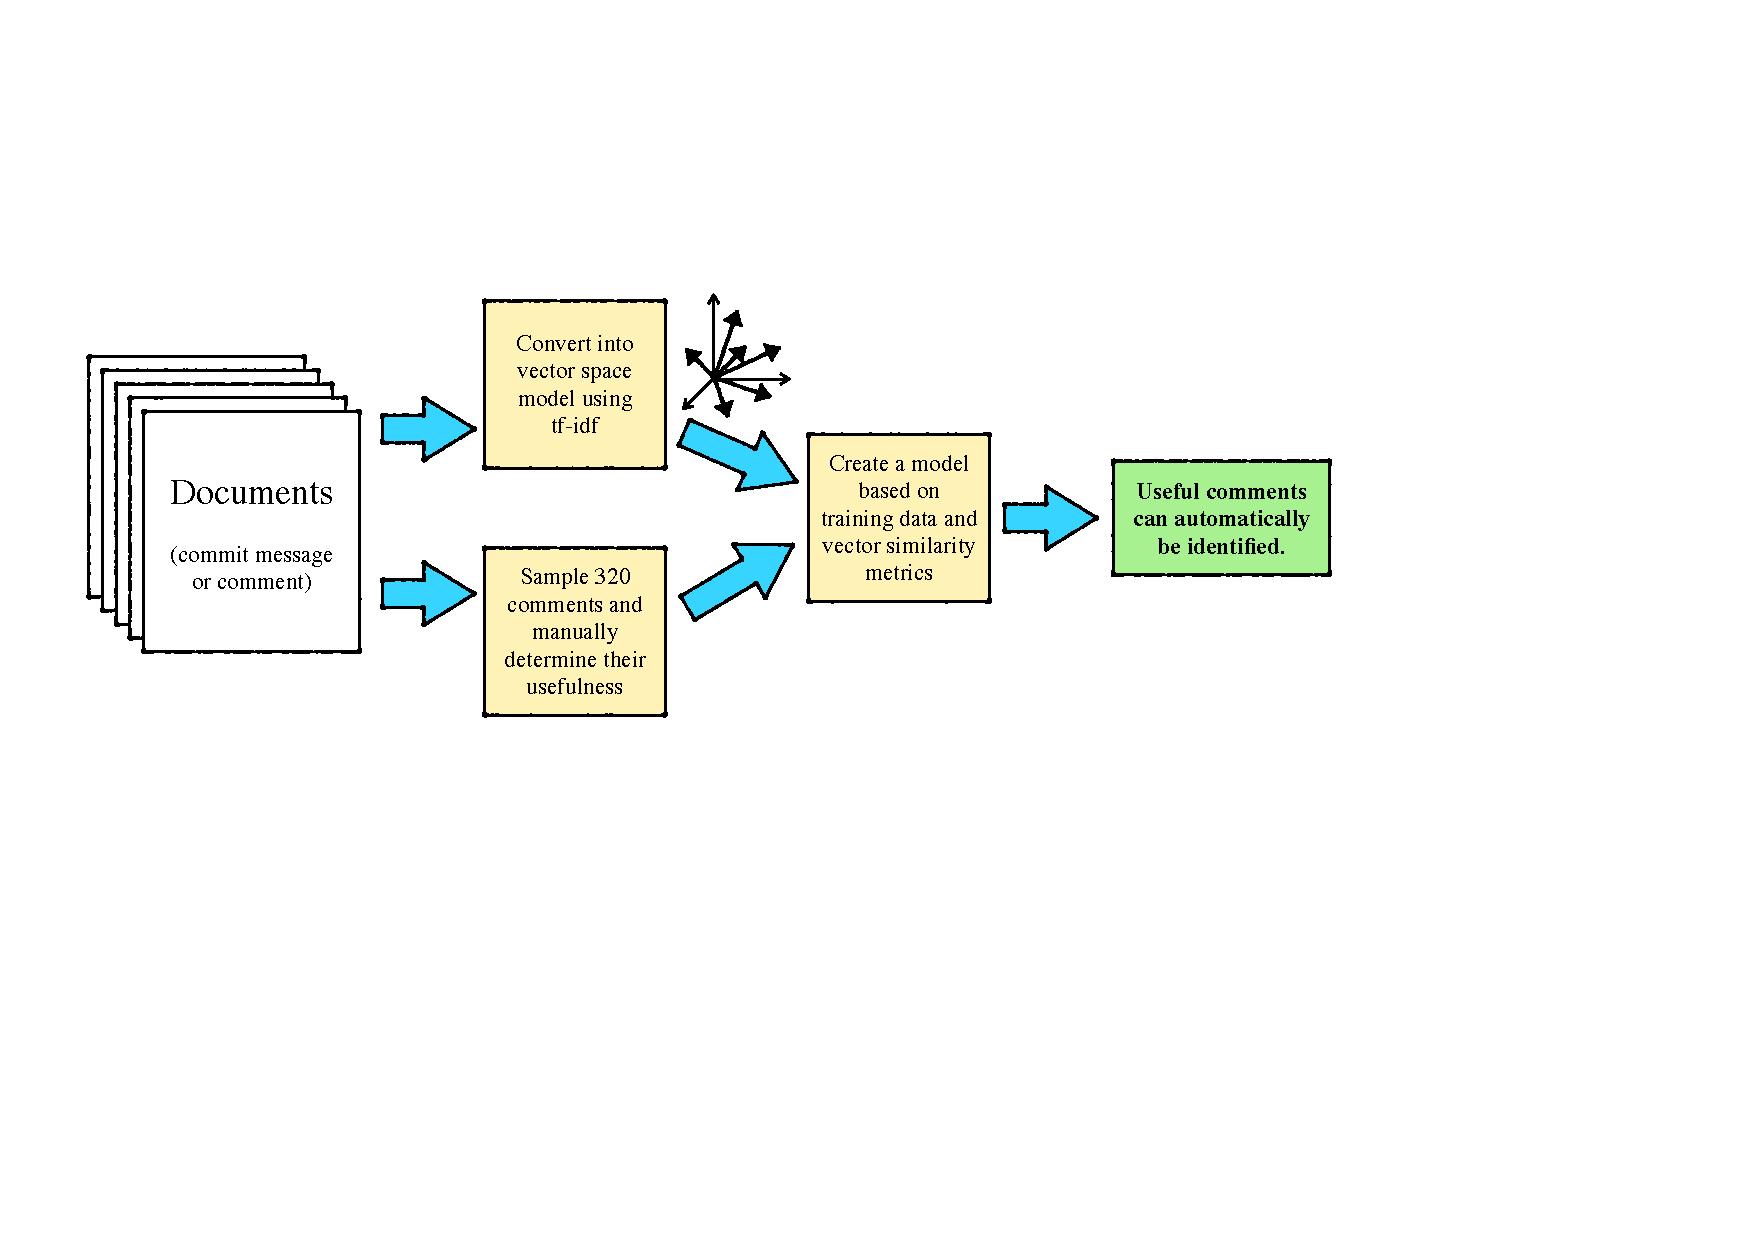
\includegraphics[width=6in]{overview}
\caption{Overview of our classification method.}
\label{fig:overview}
\end{figure*}

% where we got the data
We used the review data sets of the Qt project collected by Hamasaki et al TODO(cite properly).
Only reviews in the master branch of \texttt{qtbase} project are considered,
as it is the most active branch.

% quick structure
Each change includes a \emph{commit message} which describes what is changed.
After a change is submitted to Gerrit, reviewers can give scores to it.
The scores will determine whether the change will be accepted or not.
Reviewers can also add comments to the change, which may optionally be added to a specific line of code inside a changed file.
Majority of the comments are automatically generated by Gerrit and do not contain any user-written text.

% overview
In our classification method,
all commit messages and comments that are human-written are converted into vectors using tf--idf algorithm.
Few comments are sampled and then classified manually for use in training and validation.
A model is created from these training data, from which useful comments can automatically be identified.
This process is illustrated in Fig.\ref{fig:overview}.

\subsection{Data Preparation}

The commit messages and all comment texts are converted into vectors as part of the preparation step.
Fig. \ref{fig:preprocess} illustrates the overview of this step.
We wrote scripts in Ruby language to perform these tasks.

\begin{figure}[h]
\centering
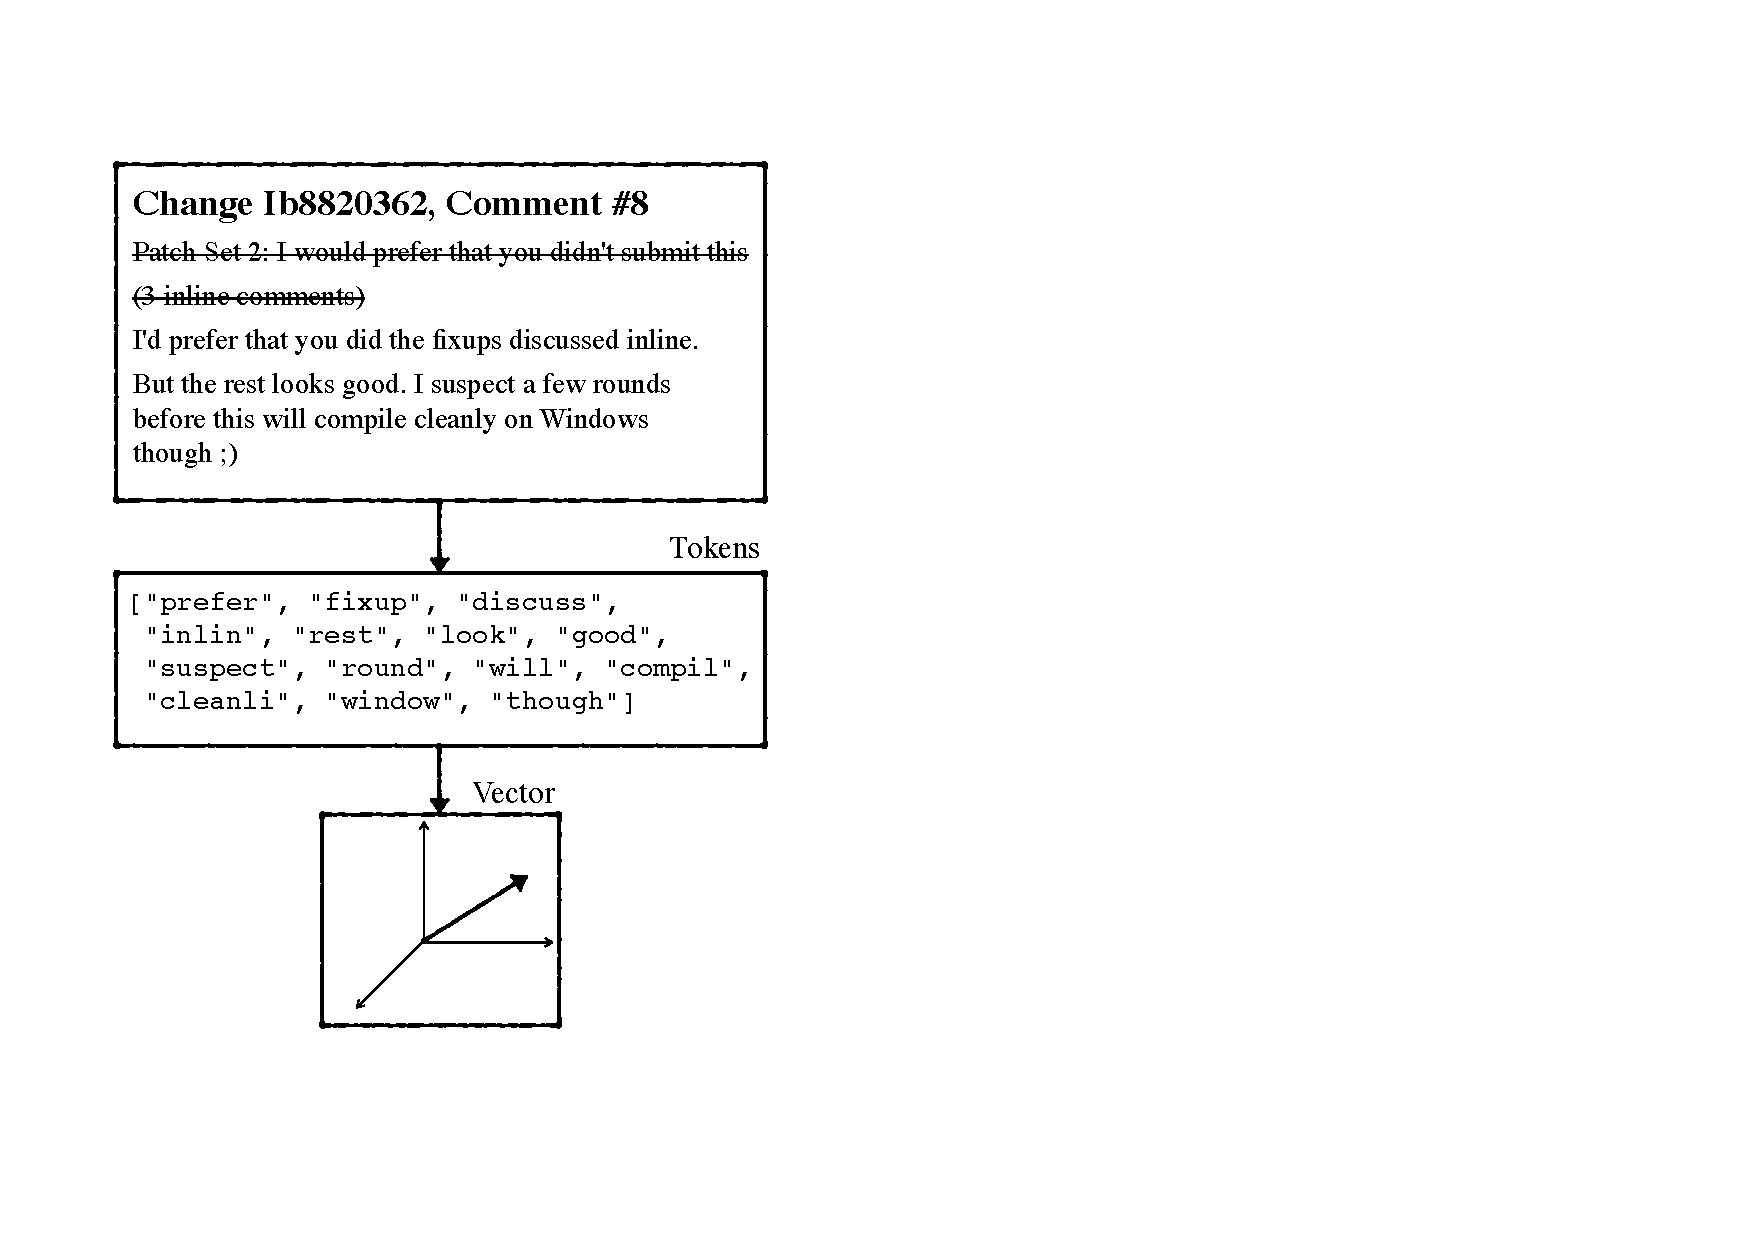
\includegraphics[width=3in]{preprocess}
\caption{The data preparation process.
Automatically generated texts are removed, remaining text is tokenized, stop words are removed, remaining tokens are stemmed,
and are converted into a vector.}
\label{fig:preprocess}
\end{figure}

\subsubsection{Removal of automatically generated text}

First, all comments by the Gerrit system, \emph{Qt Sanity Bot}, and \emph{Qt Continuous Integration System} are skipped.

% conversion into vector, wow
Next, we looked for common patterns that appeared in the comments, because it is very likely that they are automatically generated.
This is accomplished by splitting texts into lines, and for each line, searching for words that can be found in the English wordlist\footnote{The wordlist found in \texttt{/usr/share/dict/words} from Ubuntu Linux distribution is used.}.
This effectively removed the ID numbers and other non-generic terms.

Next, the lines that appears most frequently are identified.
From these lines, we then constructed the regular expression patterns,
and finally, these patterns are used to filter out automatically generated text from our data.

\subsubsection{Tokenization, stop word removal and stemming}

After the automatically generated messages are removed, we extracted the words in each document into a list of tokens by searching for alphanumeric characters including apostrophes.
Stop words from the Google stop word list\footnote{Available at \url{http://meta.wikimedia.org/wiki/Stop_word_list/google_stop_word_list#English}} are then removed.
The stemming is performed on remaining tokens using Porter stemming algorithm.
The remaining words are then combined to form a corpus of all used words.

\subsubsection{Conversion into vector}

Finally, the tf--idf algorithm is used to convert each document into a vector.


\subsection{Training Data}

We sampled 320 comments from the data set.
These samples are then classified as either useful (that is, technically contributing to the software) or not useful.
This task is carried out by three people who worked independently.

Each comment is then scored based on the number of positive answers.
For example, a comment with a score of 3 means that all three people said that it is useful,
while a comment with a score of 0 means that none of us marked it as useful.

%The score of a comment can be defined as:

%\begin{align*}
%Score_i & = \sum_{\text{reviewer } r} Review(r, i). \\
%Review(r, i) & = \begin{cases}
%	1 & \text{if } r \text{ says that the comment } i \text{ is useful,} \\
%	0 & \text{otherwise.}
%\end{cases}
%\end{align*}

\subsection{Model Generation and Validation}

% the metrics
For each comment, we computed similarity and dissimilarity metrics
between the comment text and the corresponding commit message.
We chose cosine similarity and euclidean distance as the metrics to use in model generation.

\begin{figure}[h]
\centering
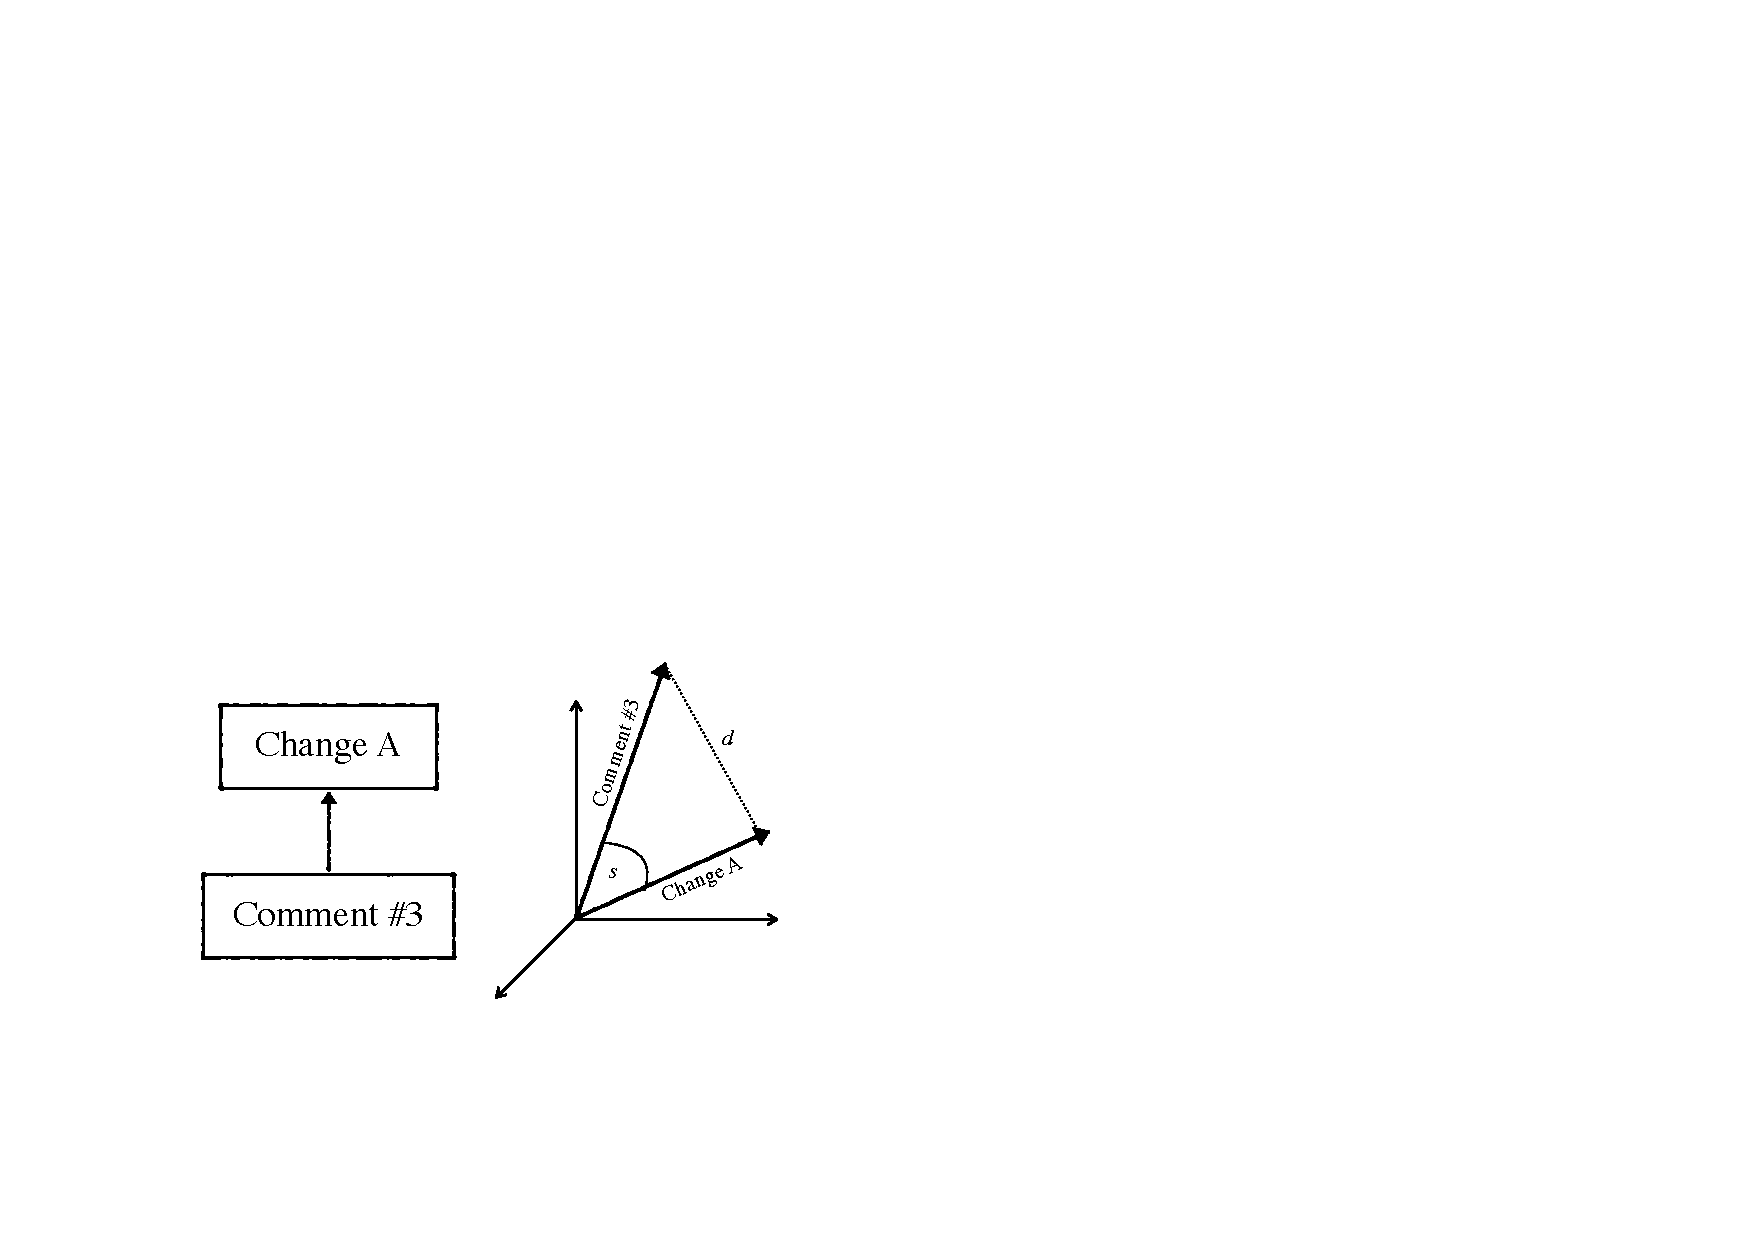
\includegraphics[width=3in]{vector}
\caption{The similarity and distance metric that is being used.}
\label{fig:vector}
\end{figure}

% assumptions in categorization
The model is based on two assumptions: that useful comments will have a $similarity \geq A \text{ and } distance \leq B$,
and that comments that are not useful will have a $ similarity \leq C \text{ and } distance \geq D$,
where $A$, $B$, $C$, and $D$ are some constant.\footnote{We also tried using the `or' operator, and found that using `and' produces better result.}

% finding parameters
To find these parameters, a brute-force approach is used.
This is possible because the set of $similarity$ and $distance$ values are discrete.
Each possible value of $A$, $B$, $C$, and $D$ are evaluated to find the constant that returns the maximum F$_1$ score.

% validation
To validate our model, 10-fold cross validation is performed.
The values of precision, recall, F$_1$ score, and accuracy are recorded and then averaged
to give the overall performance of our model.


\section{Results}

\subsection{Data Preparation}

In total, there are 6,605 changes and 72,484 comments. 25,076 comments are by the system or one of the bots.

\subsubsection{Common pattern removal}

Many common patterns are found, such as \emph{`Uploaded patch set 2.'} and \emph{`Change has been successfully cherry-picked to the staging branch as \dots'}.
The occurrences of these patterns are removed from our data set.
This leaves 36,738 comments empty, which probably means that the whole comment is automatically generated.
Only 17,275 comments and commit messages are left.

\subsubsection{Tokenizing}

After preprocessing, 393,238 tokens are generated in total. They are composed of 20,025 different words.
This means that each document will be converted into a vector of 20,025 dimensions, each dimension representing a single word.



\subsection{Training Data}

After the 320 sample comments have been labeled,
they are scored based on the number of ``yes'' given to the sample.
There were 87, 60, 51, and 122 comments with scores of 0, 1, 2, and 3, respectively.

After the similarity and distance metrics have been calculated,
these metrics appear to be able to separate the useful comments from the non-useful ones,
as can be seen in Fig.\ref{fig:scatter}.
Note that many comments have a cosine similarity metric of 0.
This is because the comment text and the corresponding commit message has no word in comment.

\begin{figure}[h]
\centering
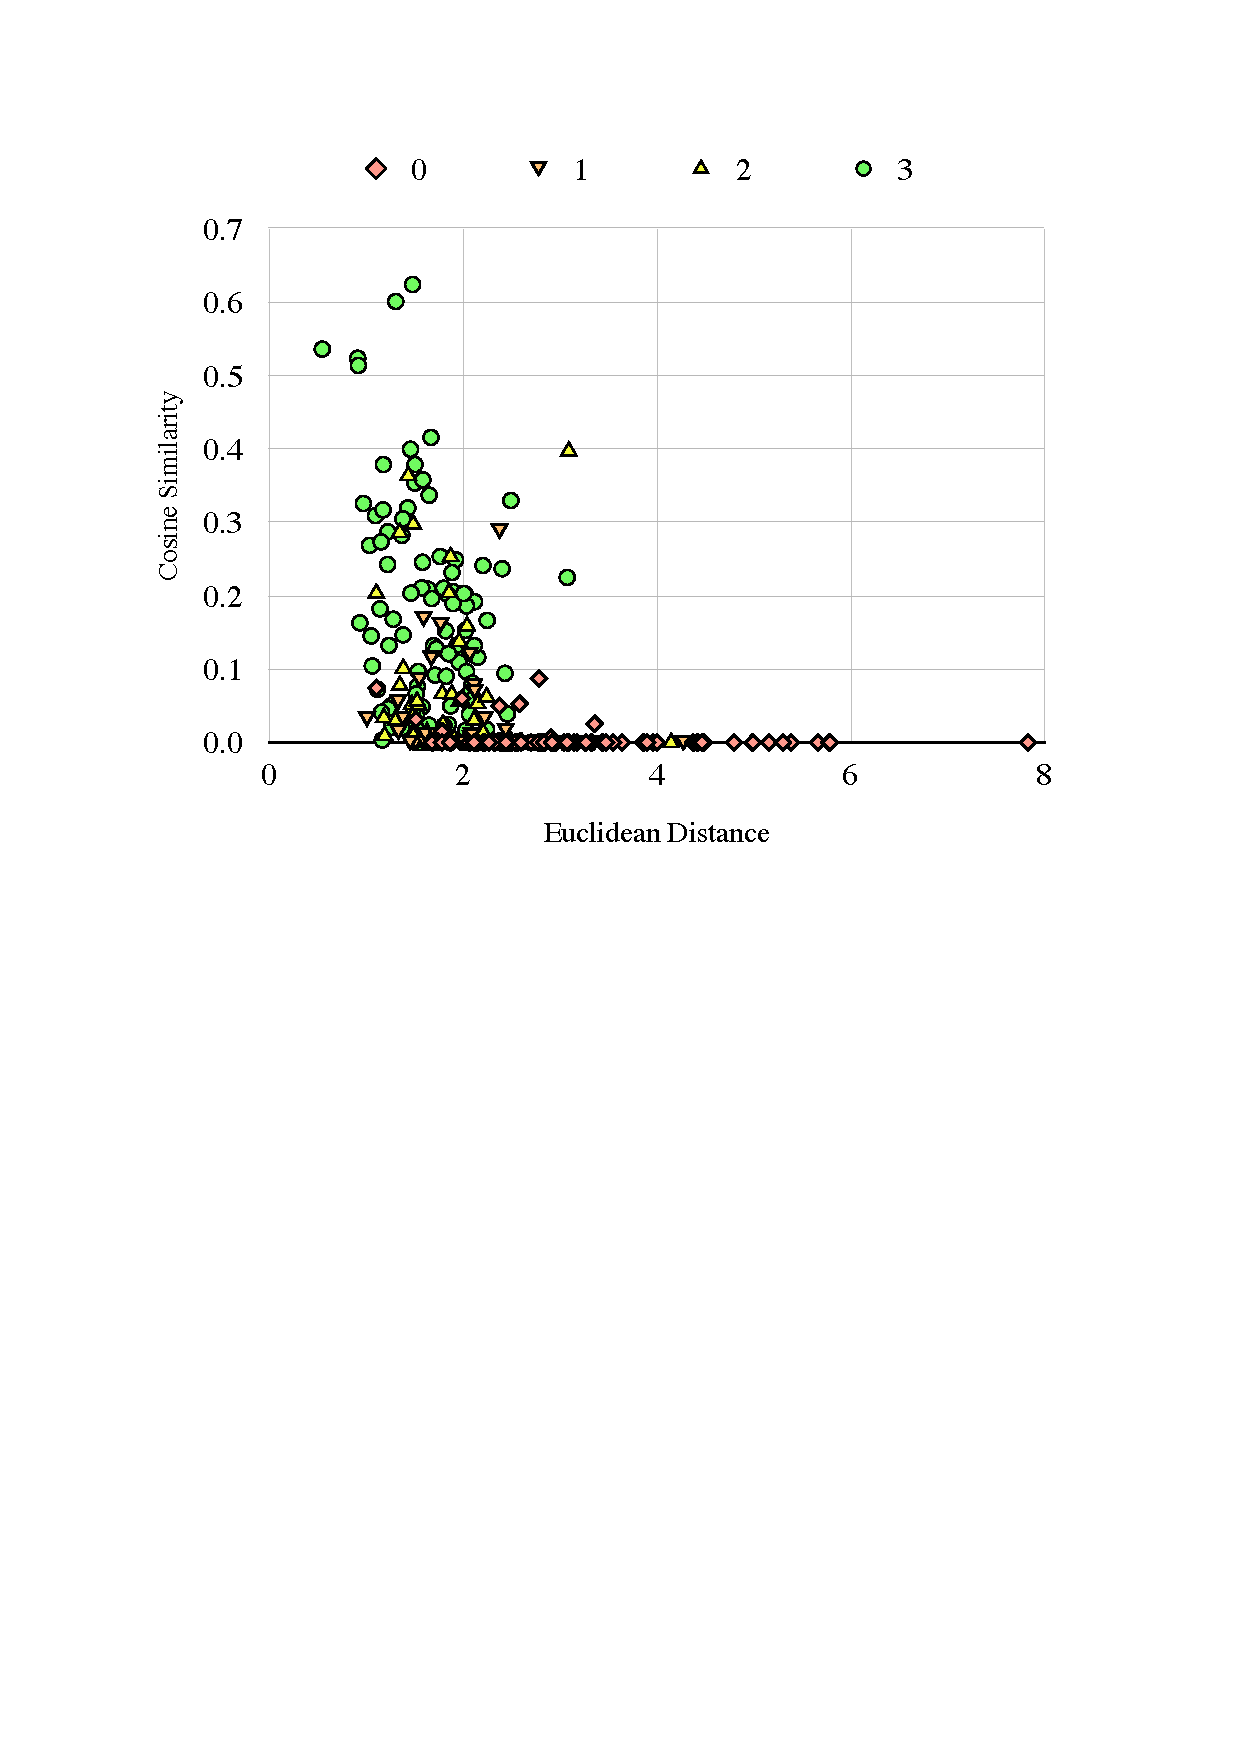
\includegraphics[width=3in]{scatter}
\caption{The similarity and distance plot of the training data.
The symbol represents the score, which ranges from 0 to 3.}
\label{fig:scatter}
\end{figure}



\subsection{Model Generation and Validation}

% the criteria that were found
From our training data,
the following criteria have been obtained that maximizes the F$_1$ score:

Criteria to find samples with score of 3 (``positive''):
\begin{gather*} similarity \geq 0.015528 \text{ and } distance \leq 2.494944
\\ \text{(F$_1$-score: 0.741313)} \end{gather*}

Criteria to find samples with score of 0 (``negative''):
\begin{gather*} similarity \leq 0.087522 \text{ and } distance \geq 2.265679
\\ \text{(F$_1$-score: 0.725389)}\end{gather*}

Note that these constant values can vary from project to project, and thus is not a universal constant.

% run result

Running our model against the training data gives us the result displayed in the following table.
In the table, \emph{Neither} means that the comment did not meet either criteria, while \emph{Overlap} means that the comment  met both ``positive'' and ``negative'' criteria.

\begin{center}
\begin{tabular}{|r|rrrr|}
\hline
& \bfseries 0 & \bfseries 1 & \bfseries 2 & \bfseries 3 \\
\hline
Negative & 69 & 23 & 7 & 6 \\
Neither & 12 & 24 & 20 & 20 \\
Overlap & 1 & 1 & 0 & 1 \\
Positive & 4 & 13 & 24 & 95 \\
\hline
\end{tabular}
\end{center}

As expected, most comments classified as \emph{negative} have score of 0 and 1,
while most \emph{positive} comments have score of 2 and 3.
However, some comments in every score were lost and classified as \emph{neither}.

% cross validation result



\section{Discussion}

% stuff






\section{Threat to Validity}


\section{Conclusion and Future Work}


\IEEEpeerreviewmaketitle

\bibliographystyle{IEEEtran}

%\bibliography{references}



% that's all folks
\end{document}


